%[Tamaño de letra 12, hoja tamaño carta, idioma español]{Documento tipo reporte}
\documentclass[12pt,letterpaper]{report}

%Interlineado del documento
\renewcommand{\baselinestretch}{1}

%Espacio parrafos
\setlength{\parskip}{5px}

%Permite configurar espaciados de forma sencilla
\usepackage{setspace}  

%Configuración de márgenes
\usepackage[left=3cm,right=3cm,top=2.5cm,bottom=2.5cm]{geometry}

%Permite el manejo de caracteres especiales en el español
\usepackage[utf8]{inputenc}
\usepackage[spanish]{babel}

%Permite manejo de ecuaciones y símbolos matemáticos
\usepackage{amsmath}
\usepackage{amsfonts}
\usepackage{amssymb}

%Permite manejo de gráficos
\usepackage{graphicx}
\graphicspath{{../figures/}}%Path de figuras

%Permite agregar sub-figuras
\usepackage{caption}
\usepackage{subcaption}

%Permite colorear texto
\usepackage{color}

%Permite manejo de múltiples columnas dentro de un mismo documento
\usepackage{multicol}

%Hipervínculos
\usepackage{hyperref}
\hypersetup{
    colorlinks=true,
    linkcolor=black,
    urlcolor=blue,
    citecolor=black}
    
%Para contraer referencias
\usepackage{cite}

%Permite que la sección bibliografía/referencias se muestre en el índice    
\usepackage[nottoc]{tocbibind}

%Símbolo de valor absoluto
\providecommand{\abs}[1]{\lvert#1\rvert}

\usepackage{tocloft}
\renewcommand{\cftfigfont}{Figura }
    
\begin{document}

%Portada del documento
\begin{titlepage}
\begin{center}

\begin{figure}
	\centering
	%Logo UAM
	
\includegraphics[scale=0.6]{variacion6Izt.png}
	\hfill
	%Logo INR
	
\includegraphics[scale=2]{INR.png}
\end{figure}

\hfill \break

\LARGE{Reporte de avances de proyecto terminal de ingeniería biomédica}

\vspace{1cm}

\rule{18cm}{0.5mm}\\
\LARGE{Aplicación de estimulación eléctrica funcional en lazo cerrado para el control contralateral de la pinza gruesa de la mano\\}
\rule{18cm}{0.5mm}

\vspace{1cm}

\Large{	\textbf{Alumno}: Enrique Mena Camilo\\
		\textbf{Matrícula}: 2153009451\\}

\vspace{1cm}

\Large{\textbf{Asesores}:\\Dr. Omar Piña Ramirez\\M.C. Jorge Airy Mercado Gutierrez}

\vspace{1cm}

\Large{26 de Enero de 2020}

\end{center}
\end{titlepage}

%INDÍCE
\pagenumbering{roman}
\tableofcontents
\newpage
\listoffigures
\newpage
\pagenumbering{arabic}

\chapter{Introducción}
%INTRODUCCIÓN
Las lesiones o daños al sistema nervioso central (SNC) suelen ocasionar alteraciones en el funcionamiento de las estructuras neuromusculares, originando condiciones de deficiencia motriz o sensorial, atrofia muscular y espasticidad. Según sea la ubicación y el grado de la lesión, serán los efectos y posibilidades de recuperación del miembro afectado. En particular, el Accidente Cerebrovascular (ACV) es un evento que reduce el flujo sanguíneo al cerebro, el cual muchas veces ocasiona hemiplejia, que es la reducción de la capacidad motriz de un lado del cuerpo.

Relacionado a las lesiones en las que el miembro superior se ve afectado, existen diferentes técnicas de rehabilitación, entre las cuales podemos encontrar las sesiones de fisioterapia, la terapia de movimiento inducido por restricción, la práctica mental con imaginación motora y sistemas de estimulación eléctrica.

La estimulación eléctrica funcional (FES, por sus siglas en inglés), es una técnica que, a partir de la aplicación de corriente eléctrica, permite la producción de potenciales de acción, y esto a su vez permite generar una contracción muscular que podría llegar a considerarse funcional\cite{Peckham2005}. Las neuroprótesis basadas en FES son dispositivos que sirven como puente entre el SNC y la zona afectada del cuerpo. Estos dispositivos buscan reemplazar o rehabilitar la función motriz dañada debido a una lesión en el SNC.

En la división de Investigación en Ingeniería Médica del Instituto Nacional de Rehabilitación ``Luis Guillermo Ibarra Ibarra'' (INR-LGII) se llevan a cabo diversos proyectos de investigación y desarrollo tecnológico, los cuales buscan desarrollar tecnología que permita aplicar nuevas técnicas de terapia de rehabilitación para personas con discapacidad motriz, o bien mejorar las técnicas ya existentes. Tal es el caso del proyecto de desarrollo de una neuroprótesis basada en FES para rehabilitación de miembro superior, que busca satisfacer las necesidades del INR-LGII en cuestiones de terapia e investigación.

Para dicho proyecto el INR-LGII desarrolló una interfaz gráfica de usuario (GUI, por sus siglas en inglés) que permite controlar los parámetros del sistema de estimulación eléctrica RehaStim 2 (HASOMED GmbH., Magdeburgo, Alemania) y el sistema de adquisición de biopotenciales Cyton Board (OpenBCI Inc., Nueva York, E.U.A.), siendo estos tres (GUI, RehaStim 2 y Cyton Board) los principales elementos de la neuroprótesis del INR-LGII. Una primera aplicación de la neuroprótesis se encuentra funcionando y se ha utilizado con sujetos sanos y pacientes del INR-LGII, aplicándoles estimulación eléctrica para generar movimientos de miembro superior. Sin embargo, actualmente el sistema opera en lazo abierto, es decir, la secuencia de estimulación se diseña y se aplica sin considerar información relevante del movimiento generado y variables relacionadas.

%\section{Planteamiento del problema}
El estado actual del proyecto del INR-LGII es la  operación en la modalidad de lazo abierto, en el cual los parámetros de la estimulación eléctrica son controlados por el experimentador quien los adapta hasta obtener el patrón específico útil para el sujeto en rehabilitación. Esto causa una dependencia del experimentador para la operación del sistema, y limita su utilidad para objetivos de rehabilitación, ya que no considera variables intrínsecas del paciente, como la intención de movimiento o actividad residual, que podrían contribuir a la modulación de los parámetros de estimulación y el movimiento resultante.

%\section{Justificación}
Ante esta problemática en la que se encuentra la neuroprótesis desarrollada en el INR-LGII, los sistemas involucrados trabajan sin tener retroalimentación entre ellos, surge la necesidad de implementar alguna aplicación que permita la interacción entre sistemas y que además permita la participación del paciente de forma activa en la terapia.

Por ello, este proyecto plantea desarrollar una aplicación en lazo cerrado que permita la participación activa del paciente (a partir de señales de sEMG (electromiografía de superficie) del brazo sano) en la terapia de rehabilitación basada en FES, llevando a cabo una modulación de la estimulación eléctrica que permita la ejecución, en el brazo afectado, de los movimientos involucrados en el agarre de un objeto (flexión y extensión de los dedos). Un sistema con estas características permitiría al sujeto tener el control sobre los movimientos de la mano contralateral, y además disminuiría la dependencia del experimentador en el proceso de la terapia.

Trabajos como los documentados en \cite{Zhou2018} \cite{Kim2015} \cite{Yi2013} \cite{Fonseca2019}, son prueba de que un control contralateral (también llamado en ocasiones entrenamiento en espejo) basado en sEMG es útil para llevar a cabo tareas motoras funcionales basadas en FES, siendo el sEMG utilizado para iniciar algún patrón FES o bien para modular los parámetros de esta.

Otros trabajos como \cite{Salchow2016} \cite{Sun2014} \cite{Woods2018}, muestran la posibilidad de crear sistemas en lazo cerrado que se ejecutan en tiempo real utilizando el dispositivo de estimulación eléctrica RehaStim 2 (o una versión anterior a esta), el cual es el dispositivo de estimulación eléctrica con el que cuenta la neuroprótesis del INR-LGII.

%\section{Hipótesis}
Considerando los trabajos antes mencionados, se formula la hipótesis de este proyecto de la siguiente manera: al integrar los diferentes bloques de un sistema de estimulación eléctrica funcional dentro de una plataforma de software con herramientas de tiempo real, se logrará implementar una aplicación FES en lazo cerrado que permita llevar a cabo en línea la adquisición y procesamiento de señales de sEMG en línea, como parte de un esquema de control contralateral de movimientos de la mano.

%\section{Objetivos}
Siendo el objetivo general de este proyecto diseñar e implementar un esquema de control contralateral para miembro superior, que permita la modulación de la amplitud de estimulación eléctrica a partir de señales de sEMG. Teniendo como objetivos particulares los siguientes:

\begin{itemize}
	\item Desarrollar y evaluar un bloque de adquisición dentro de Simulink\textregistered \;  (The MathWorks Inc., Natick, MA, E.U.A.) que permita la recepción de datos seriales de un dispositivo multicanal de registro de biopotenciales.
	\item Desarrollar un algoritmo de identificación de los movimientos de flexión y extensión de la mano a través de señales de sEMG.
	\item Diseñar e implementar un esquema de control que permita la modulación continua de la amplitud de la estimulación eléctrica para control del movimiento de la mano, en combinación con el algoritmo identificador de movimientos.
\end{itemize}


\chapter{Marco teórico}
%Marco Teórico

\section{Estimulación eléctrica funcional}
La estimulación eléctrica funcional es la aplicación de corriente eléctrica a tejido excitable para auxiliar o restaurar funciones que se han perdido en individuos con daños neurológicos. El propósito de la intervención FES es habilitar funciones que se han perdido en individuos con daño al sistema nervioso mediante la sustitución o asistencia a las habilidades voluntarias de dichos individuos. En las aplicaciones FES la estimulación es requerida para lograr una función deseada, por lo tanto, los sistemas FES usualmente se diseñan para ser controlados a partir de señales relacionadas a la actividad o intención del propio usuario. Los dispositivos FES que son usados para sustituir una función neurológica que se ha perdido son comúnmente llamados neuroprótesis \cite{Peckham2005}.

En la Figura \ref{Figura: FES} se puede observar que al aplicar estimulación eléctrica en el músculo, este responderá a dicha estimulación realizando una contracción, la cual puede ir disminuyendo durante el periodo de estimulación.

%Figura FES
\begin{figure}[htbp]
	\centering
	\begin{subfigure}[htbp]{0.4\textwidth}
		\centering
		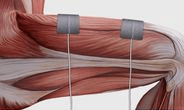
\includegraphics[width=\textwidth]{FES1.png}
		\caption{Músculo sin estimulación eléctrica.}
		\label{Figura: FES1}
	\end{subfigure}
	\hfill
	\begin{subfigure}[htbp]{0.4\textwidth}
		\centering
		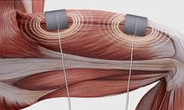
\includegraphics[width=\textwidth]{FES2.png}
		\caption{Músculo con estimulación eléctrica.}
		\label{Figura: FES2}
	\end{subfigure}
	\caption[Efecto de aplicar estimulación eléctrica en músculo]{Efecto de aplicar estimulación eléctrica en músculo.}
	\label{Figura: FES}
\end{figure}

\section{Neuroprótesis}
Una neuroprótesis es un dispositivo compuesto de elementos que permiten utilizar la estimulación eléctrica como interface directa con el sistema nervioso, y cuyo fin es reemplazar o asistir alguna función deteriorada del sistema nervioso, deficiencia que suele ser el resultado de una enfermedad o lesión. Las neuroprótesis comúnmente actúan como un puente entre elementos funcionales del sistema nervioso central y los nervios o músculos sobre los cuales se ha perdido control (Figura \ref{Figura: NeuroP}) \cite{Finn2003}\cite{Popovic2008}.

%Una neuroprótesis es un dispositivo que proporciona ráfagas cortas de impulsos eléctricos al sistema nervioso central o periférico a través de electrodos superficiales, para lograr producir funciones sensoriales o motoras. Estos dispositivos buscan sustituir o asistir una función dañada debido a una lesión o enfermedad en el sistema nervioso \cite{Popovic2008} \cite{Popovic2015}.

En general, existen dos tipos de neuroprótesis: a) las neuroprótesis autónomas, las cuales son sistemas autocontenidos que imitan las funciones de una contraparte biológica, y b) las neuroprótesis por comando, las cuales son sistemas que reemplazan o asisten una función sensitiva o motora que se ha perdido o disminuido. Estas últimas están compuestos por un sistema de control que interpreta la intención del usuario, utilizan sensores para detectar el estado del sistema, genera la activación del sistema motor o sensorial del usuario, y proporciona una retroalimentación al usuario \cite{Popovic2015}.

Las neuroprótesis motoras, las cuales son un ejemplo de neuroprótesis por comando, son sistemas que asisten a personas que han sufrido algún tipo de lesión en la médula espinal o cerebro. Estas neuroprótesis pueden actuar directamente en el sistema nervioso central, en el sistema nervioso periférico, o bien, en una combinación de ambos, tiendo como objetivo principal realizar contracciones musculares que generen movimientos relevantes para el sujeto \cite{Popovic2015}.

%Figura Neuroprótesis
\begin{figure}[htbp]
	\centering
	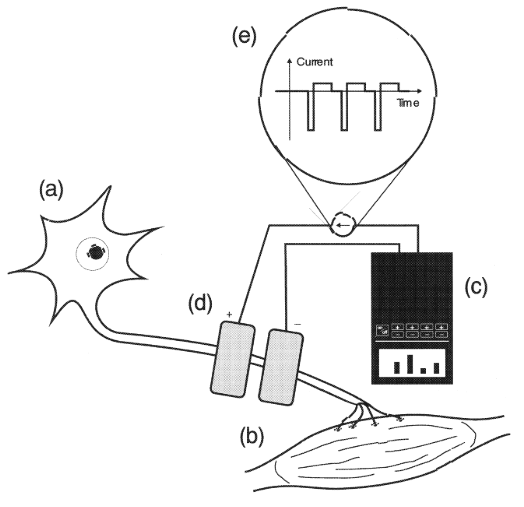
\includegraphics[width=0.4\textwidth]{NeuroP.png}
	\caption[Estimulación directa a una neurona motora]{Estimulación directa a una neurona motora. La neurona motora (a) es la responsable de generar señales de activación que son transmitidas a la correspondiente fibra muscular (b). Posterior a un accidente cerebrovascular o una lesión de la médula espinal, el músculo queda incomunicado con el sistema nervioso central. Una neuroprótesis (c) inyecta corriente eléctrica dentro del axón de la célula (d), corriente formada por un tren de pulsos negativos y positivos (e) que producen potenciales de acción que activan la fibra muscular. Recuperado de \cite{Popovic2008}.}
	\label{Figura: NeuroP}
\end{figure}

\section{Señales de comando y retroalimentación}\label{Seccion: ComRetro}

Una neuroprótesis por comando requiere de dos tipos de señales esenciales para lograr su correcto funcionamiento, las cuales son las señales de comando y las señales de retroalimentación \cite{Popovic2015}. En la Figura \ref{Figura: CompNeuroP} se pueden observar de forma general las conexiones que dichas señales realizan con el resto de los componentes de una neuroprótesis.

\begin{figure}[htbp]
\centering
	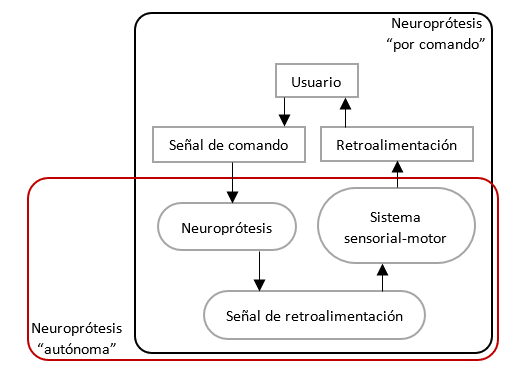
\includegraphics[width=0.6\textwidth]{CompNeuroP_ESP.png}
	\caption[Componentes generales de una neuroprótesis]{Componentes generales de una neuroprótesis autónoma (recuadro rojo) y por comando (recuadro negro). Adaptado de \cite{Popovic2015}.}
	\label{Figura: CompNeuroP}
\end{figure}

%\subsection{Señal de comando}
Las señales de comando son aquellas se usan para activar, desactivar o modular determinadas funciones o acciones dentro del sistema de control de la neuroprótesis. Estas señales pueden generarse de diversas formas, sin embargo, como se ilustra en la Figura \ref{Figura: CompNeuroP}, suelen ser generadas por el usuario \cite{Popovic2015}. Ejemplos de dichas señales podrían ser la acción de presionar un botón que indique a la neuroprótesis el momento de inicio y fin de la estimulación eléctrica; o bien, un conjunto de señales fisiológicas que permitan identificar la tarea que busca realizar el individuo.

%\subsection{Señal de retroalimentación}
En la Figura \ref{Figura: CompNeuroP} se puede observar que la señal de retroalimentación es aquella señal que se genera como salida de la neuroprótesis, es decir, la estimulación eléctrica que se inyecta al sistema sensorial-motor del usuario; sin embargo, también se puede observar una retroalimentación dirigida hacia el usuario, la cual puede ser una contracción muscular activada por el comando del usuario o el movimiento de algún sistema robótico \cite{Popovic2015}. Esta última retroalimentación es la que suele ser relevante para el sistema de control de la neurorótesis.

Aclarado el concepto de retroalimentación que se abordará en el presente trabajo, se puede definir a las señales de retroalimentación como un tipo de señales que brindan información relacionada a la respuesta del sujeto ante un determinado comando. Dichas señales son útiles para indicar al sistema de control si la respuesta del sujeto se apega a la respuesta esperada, y en caso contrario modificar los parámetros de dicho sistema para conseguir la respuesta esperada \cite{Wright2016}. Estas señales de retroalimentación se pueden obtener de diversas maneras, las cuales se abordan en la sección \ref{Seccion: Retro}.

\section{Esquemas de control}
Existen dos tipos de control importantes dentro de las aplicaciones de una neuroprótesis, los cuales se diferencian esencialmente en los tipos de señales que ocupan. En la Figura \ref{Figura: EsqCont} se ilustran a grandes rasgos las diferencias entre ambos esquemas de control.

\begin{figure}[htbp]
\centering
	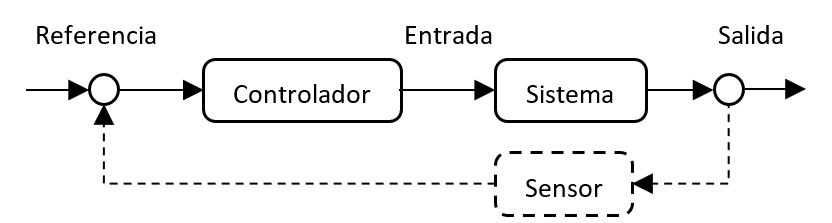
\includegraphics[scale=0.7]{EsquemasControl_ESP.png}
	\caption[Esquema general de control en lazo abierto y control en lazo cerrado]{Esquema general de control en lazo abierto y control en lazo cerrado. El control en lazo abierto se ilustra con una línea sólida. El control en lazo cerrado se lleva a cabo cuando se incluye el elemento sensor, el cual se ilustra con una línea discontinua. Adaptado de \cite{Wright2016}.}
	\label{Figura: EsqCont}
\end{figure}

%\subsection{Control en lazo abierto}
En el control en lazo abierto (línea sólida de la Figura \ref{Figura: EsqCont}) se genera un comando a la línea de base (estado o valor inicial del sistema), esperando que este comando produzca la salida correcta. Aquí no existe una medición de la salida generada, por lo cual tampoco existe alguna medición del error que pudiera utilizarse como mecanismo para la modulación del comando que se genera \cite{Wright2016}. En este esquema de control, el experimentador es el encargado de modificar los parámetros del sistema hasta conseguir una salida apegada a la salida esperada.

%\subsection{Control en lazo cerrado}
El control en lazo cerrado (línea sólida más línea discontinua de la Figura \ref{Figura: EsqCont}) requiere de la inclusión de algún elemento sensor en el sistema que se desea controlar. Este control retroalimentado genera un comando a la línea de base y el elemento sensor mide la salida del sistema en respuesta al comando. Esta medición de la salida puede utilizarse para determinar diferencias entre la salida esperada y la real, generando así una señal de error que puede utilizarse como retroalimentación hacia el controlador para realizar modificaciones en los comandos generados \cite{Wright2016}.

%\subsection{Control adaptativo}
Otro esquema de control capaz de implementarse en aplicaciones de neuroprótesis (tanto en lazo abierto como en lazo cerrado) es el control adaptativo. Este esquema de control utiliza sensores para medir la entrada y salida del sistema, utilizando dichas métricas para ajustar el controlador en respuesta a las perturbaciones en el entorno de control o el sistema controlado, buscando siempre mantener un nivel de desempeño preestablecido. Una ventaja de este tipo de control es que se pueden desarrollar estrategias de control sin requerir de un conocimiento completo del sistema que se va a controlar, sin embargo, esto provoca que los controladores adaptativos rara vez sean óptimos \cite{Wright2016}.

\section{Algoritmos de control}
Existe una gran variedad de algoritmos de control que suelen ser usados dentro de las neuroprótesis, sin embargo, para este trabajo sólo se abordaran 3 algoritmos de control.

%\subsection{Control on-off}
El control on-off es un algoritmo en el que se monitorea si una determinada variable de control se encuentra por encima o por debajo de un determinado umbral, con lo cual se suelen activar o desactivar determinadas funciones del sistema de control \cite{Wright2016}. En aplicaciones FES, este tipo de control suele utilizarse para activar una secuencia predefinida de estimulación eléctrica. Este algoritmo de control también suele utilizarse configurando dos umbrales por los cuales la variable de control puede pasar, por ejemplo, para el control de temperatura de una incubadora neonatal, en la cual se requiere que la temperatura de esta se encuentre dentro de un intervalo específico, en este caso, el control on-off podría aplicarse de la siguiente manera: si la temperatura se encuentra por encima del límite superior de temperatura, la calefacción se apaga; mientras que si la temperatura se encuentra por debajo del límite inferior de temperatura, la calefacción se enciende \cite{Wayne2003}.

%\subsection{Máquina de estados finitos (FSM)}
Una máquina de estados finitos (FSM, por sus siglas en inglés) es un modelo de sistema que puede considerarse como una implementación más compleja del control on-off. En este modelo, la medición de una variable del sistema en combinación con el estado actual de la misma, desencadenan una transición de estado, la cual a su vez genera una serie de acciones en el sistema que se está controlando. Debido a que este tipo de modelo suele ser periódico, puede ser útil para realizar transiciones de estado en respuesta al tiempo \cite{Wright2016}. En aplicaciones FES, las acciones generadas debido a la transición de estados suelen asociar al inicio o fin de la estimulación eléctrica, los periodos de rampa en el patrón de estimulación, o bien los periodos de modulación de la estimulación eléctrica.

%{\color{red}\subsection{Control proporcional}}
El control proporcional (también conocido como control P), es un tipo control en el cual se aplica una corrección a la variable de control, la cual es proporcional entre el valor deseado y el valor real. Este tipo de control es más complejo que el control on-off, pero a su vez es más simple que un control proporcional-integral-derivativo (PID). Este tipo de control suele ser útil para llevar a cabo el control de sistemas que cuentan con un tiempo de respuesta rápido. En este tipo de control, la salida es proporcional a la señal de error (diferencia entre el valor esperado y el real), proporción que está definida por la Ecuación \ref{Ecu: Recta}, donde $P$ representa la salida proporcional, $K_{p}$ representa la ganancia proporcional, $e(t)$ representa el error instantaneo en el momento $t$, $p_{0}$ representa la salida con cero errores \cite{Wayne2003}. En aplicaciones FES, este tipo de control se ha mostrado útil para llevar a cabo la modulación de algún parámetro de estimulación eléctrica (como puede ser la amplitud o el ancho de pulso), donde la determinación de los factores $K_{p}$ y $p_{0}$ serán los responsables directos del grado de desempeño de la modulación \cite{Zhou2018}.

\begin{equation}
	P = K_{p} e(t) + p_{0}
	\label{Ecu: Recta}
\end{equation}

\section{Retroalimentación}\label{Seccion: Retro}
Como se explicó en la sección \ref{Seccion: ComRetro}, una señal de retroalimentación es aquella que brinda información al sistema sobre los efectos ante un determinado comando. Estas señales se pueden implementar de más de una forma dentro de una neuroprótesis, por ejemplo, la observación visual de la acción realizado por algún actuador robótico de una una interfaz cerebro-computadora (comúnmente conocido como neurofeedback), la adquisición de una señal bioeléctrica durante un periodo de estimulación eléctrica, o bien la medición de algún elemento sensor que proporcione información sobre el estado del efector o actuador \cite{Wright2016}.

Otro ejemplo de retroalimentación en un sistema de neuroprótesis es el biofeedback, una técnica de retroalimentación donde no se requiere de elemento sensor en el efector o actuador del sistema, ya que consiste en permitir al individuo usuario de la neuroprótesis aprender a cambiar su actividad fisiológica con el fin de mejorar el rendimiento del sistema \cite{Yucha2008}.

\section{Electromiografía de superficie}
La electromiografía (EMG) se define como la detección y análisis de la señal eléctrica derivada de la actividad contráctil de los músculos. El EMG puede detectarse directamente mediante la inserción de electrodos en las fibras musculares, o de forma indirecta colocando electrodos de superficie en las zonas de la piel localizadas justo encima del tejido muscular. A este último método se le suele conocer como electromiografía de superficie (sEMG, por sus siglas en inglés), el cual, al ser un método de detección no invasivo y permitir obtener información sobre la activación muscular, como la intensidad de la contracción muscular, la manifestación de la fatiga muscular y el reclutamiento de unidades motoras, se ha convertido en un método muy popular en la investigación.

\subsection{Procesamiento del sEMG}
La actividad mioeléctrica en la superficie de la piel se encuentra dentro de un ancho de banda limitado que suele estar desde los 15 hasta los 400 Hz, con amplitudes dentro del rango de $\mu V$ o $mV$, dependiendo de la intensidad de la contracción muscular \cite{Cavalcanti-Garcia2009}.

La detección de la actividad mioeléctrica se realiza mediante el uso de un amplificador diferencial, el cual debe tener conectadas las entradas a un par de electrodos situados a lo largo de la dirección de la fibra muscular a sensar, y un tercer electrodo de referencia situado en el hueso más cercano a la fibra. Una vez detectada de forma eficaz la actividad mioeléctrica, esta debe someterse a un filtro analógico anti-aliasing y posteriorme al proceso de conversión analógico-digital que permitirá se realice el procesamiento digital de la señal \cite{Cavalcanti-Garcia2009}.

Usualmente se suele utilizar un filtro pasa banda con frecuencias de corte similares a las que componen la actividad mioeléctrica (15-400 Hz), acompañado de un filtro notch digital que permita atenuar la interferencia provocada por la línea \cite{Cavalcanti-Garcia2009}.

\subsection{Descriptores de amplitud del sEMG}
Existen diferentes indicadores que pueden ser utilizados para estimar la amplitud del sEMG, tal es el caso de la amplitud pico a pico, la cual nos proporciona un valor instantáneo de la amplitud del sEMG. Sin embargo, este no es un indicador robusto de la amplitud de la señal de sEMG \cite{Cavalcanti-Garcia2009}.

Los descriptores de amplitud de sEMG más comunes son la promediación de muestras rectificadas o elevadas al cuadrado de sEMG crudo a lo largo de una determinada tarea motora. Estos descriptores se conocen como el valor rectificado promedio (ARV o MAV, por sus siglas en inglés)(Ecuación \ref{Ecu: ARV}) y el valor cuadrático medio (RMS, pos sus siglas en inglés)(Ecuación \ref{Ecu: RMS}). Dichos descriptores suelen usarse para estimar las variaciones temporales de la amplitud del sEMG en ventanas cortas entre 250 ms o 500 ms \cite{Cavalcanti-Garcia2009}.

\begin{equation}
	ARV = \frac{1}{N} \sum_{n=1}^{N} \abs{EMG[n]}
	\label{Ecu: ARV}
\end{equation}

\begin{equation}
	RMS = \sqrt{\frac{1}{N} \sum_{n=1}^{N} EMG[n]^{2}}
	\label{Ecu: RMS}
\end{equation}

Estos descriptores de amplitud suelen proporcionar información similiar, la gran diferencia entre ellos se encuentra en la función de densidad de probabilidad (PDF, por sus siglas en inglés) que generan, donde el RMS suele ser un descriptor con PDF Gaussiana, mientras que el ARV suele ser una descriptor con PDF Laplaciana. En general, se suele utilizar el RMS debido que teóricamente la PDF de sEMG es Gaussiana, sin embargo, existen trabajos que han demostrado que en la práctica la PDF de sEMG es más cercana a una PDF Laplaciana, caso en el cual es recomendable utilizar el ARV como descriptor \cite{Clancy1999}\cite{Phinyomark2013}.

\chapter{Antecedentes}
\section{Desarrollos previos al proyecto}
{\color{red}Peña: ¿Dónde están publicados los trabajos realizados en el INR?}

En el INR se han realizado trabajos previos relacionados al desarrollo de la neuroprótesis, los cuales han logrado que dicho sistema sea funcional y se pueda ocupar en pacientes del propio instituto. Este trabajo incluye una plataforma de software para control y configuración de la neuroprótesis, la implementación de una aplicación FES en lazo abierto comandada por EEG, y un sistema prototipo de adquisición de biopotenciales.

\subsection{Plataforma de software para neuroprótesis}
Consiste en una GUI implementada en la herramienta GUIDE de MATLAB®, la cual consta de 4 pantallas que en conjunto permiten, hasta el momento: a) realizar el registro de datos de un paciente o usuario en el que se probará el dispositivo, b) realizar el entrenamiento de un clasificador de movimientos voluntarios, c) ejecutar una aplicación FES en lazo abierto, o bien d) experimentar con los parámetros del estimulador y el sistema de registro de biopotenciales para determinar el patrón de estimulación óptimo para el paciente. Esta plataforma realiza una conexión a dispositivos comerciales: Rehastim 2 (Hasomed GmbH, Alemania) para estimulación eléctrica, y Cyton Board (OpeBCI Inc, E.E.U.U.) para adquisición de biopotenciales) que permiten la integración de las funciones de la NP.

\subsection{Aplicación FES en lazo abierto}
La aplicación FES, que se encuentra inmersa en la plataforma de software para la neuroprótesis, está basada en una Interfaz Cerebro-Computadora. Dicha aplicación le muestra al sujeto una serie de 5 movimientos predefinidos, dentro de los cuales el sujeto debe seleccionar alguno cerrando los ojos. Una vez seleccionado y confirmado el movimiento objetivo, el sistema envía una secuencia de pulsos de estimulación eléctrica para asistir al sujeto a realizar el movimiento elegido. En esta aplicación el patrón de estimulación eléctrica está predeterminado antes de iniciar la aplicación.

\subsection{Sistema prototipo de adquisición de biopotenciales}
Sistema que consta del convertidor analógico digital ADS1299 y el microcontrolador MSP432P401R. Es un sistema que presenta ventajas respecto al sistema comercial utilizado en trabajos anteriores basados en OpenBCI, principalmente una frecuencia de muestreo de 1 kHz por canal, la cual es útil para fines de control con sEMG \cite{Lenzi2012}\cite{Lenzi2011}\cite{Raafat}. Además, el prototipo utiliza una conexión USB para la transmisión de datos, la cual, a diferencia de la conexión bluetooth con la que cuenta el dispositivo de OpenBCI, permite una mayor tasa de transmisión de datos (460800 bps, contra 115200 bps). %y evita la pérdida de datos que se presentaba en el sistema comercial por fallas en la conexión bluetooth.

El sistema prototipo de adquisición será útil para fines de este proyecto, ya que gracias a la interfaz gráfica desarrollada previamente para dicho sistema, se tiene la posibilidad de ajustar los parámetros de adquisición de tal forma que nos permitirá obtener una señal de sEMG de mejor calidad que con el sistema OpenBCI.

\section{Sistemas FES existentes}
En el Cuadro ~\ref{Cuadro:Sistemas FES} se muestran los trabajos revisados que proporcionan información de interés para lograr los objetivos de este proyecto. Dentro de los campos que se destacan de dichos trabajos se encuentran: la aplicación, debido a que se buscaron trabajos que asistan el funcionamiento de las extremidades, en especial de miembro superior; el dispositivo de estimulación, ya que se buscaron trabajos que utilizaran el mismo dispositivo a utilizar en este proyecto o bien sus versiones anteriores; la implementación del esquema de control, esto debido a que se buscaron sistemas que aprovecharan el entorno de Simulink, ya que el controlador del dispositivo de estimulación eléctrica a emplear (Rehastim2) está desarrollado en dicha plataforma; y finalmente, las señales que dichos sistemas utilizaron para realizar la retroalimentación del sistema y la activación de los comandos.

De estos trabajos se puede rescatar que, al realizar un entrenamiento en espejo donde sea un miembro sano el que controla la estimulación eléctrica aplicada al miembro dañado, se lograrán disminuir los artefactos generados por esta al momento de registrar EMG, o bien serán nulos si se ocupa una técnica de cuantificación de movimiento de origen no bioeléctrico \cite{Salchow2016}. También, se destaca que para realizar una terapia de asistencia para apertura y cierre de mano es necesario tener indicadores del estado actual de la mano y del estado del objeto sobre el que se quiere realizar la acción \cite{Simonsen2017}. Adicional a esto, se ha demostrado que implementar una máquina de estados finitos para el control de una neuroprótesis es algo viable y que permite la comprensión rápida, por parte del usuario, del funcionamiento del esquema de control \cite{Sun2014}. Por último, se destaca que, de lograr integrar todos los componentes del esquema de control en una misma plataforma, se pueden realizar aplicaciones que presenten un funcionamiento en tiempo real o muy cercano a este \cite{Salchow2016}\cite{Sun2014}\cite{Woods2018}.

%Cuadro de revisión bibliográfica
\begin{table}[hbt]
	\centering
	\begin{tabular}{|p{25mm}|p{35mm}|p{25mm}|p{40mm}|p{35mm}|}
	\hline
	\textbf{Referencia} & \textbf{Aplicación} & \textbf{Dispositivo de estimulación} & \textbf{Señales de comando y retroalimentación} & \textbf{Implementación del sistema de control}\\ 
	\hline
	%\cite{Salchow2016}
	(Salchow, 2016) & Entrenamiento en espejo para posturas de mano & RehaMove Pro & Electromiografía, movimiento de mano & MATLAB/Simulink\\
	\hline
	%\cite{Sun2014}
	(Sun, 2014) & Recuperación de funciones de miembro superior & RehaStim1 & Acelerómetro & Simulink\\
	\hline
	%\cite{Simonsen2017}
	(Simonsen, 2017) & Asistencia para apertura y cierre de mano & STMISOLA & Posición del objeto, posición de la mano & MATLAB\\
	\hline
	%\cite{Woods2018}
	(Woods, 2018) & Asistencia en miembro inferior para ciclisco & RehaStim 1 & Mecanomiografía, fuerza aplicada a pedales, posición del cigüeñal & Simulink\\
	\hline
	\end{tabular}
	\centering
	\caption{Revisión de sistemas FES reportados en la literatura con aplicaciones similares a las de este proyecto.}
	\label{Cuadro:Sistemas FES}
\end{table}

{\color{red}Agregar revisión de métodos de procesamiento y control para aplicaciones de FES contralateral en otro cuadro}

\chapter{Metodología}
\section{Sistema propuesto}
Para este proyecto se planteó un sistema que implementa un lazo cerrado utilizando biofeedback. El sistema consiste en la adquisición de dos canales de sEMG, del brazo izquierdo, los cuales son procesados y sirven como entrada de un sistema de control que realiza la modulación de la amplitud de dos canales de estimulación eléctrica en el brazo derecho. Este sistema implementa un control contralateral para realizar un entrenamiento en espejo de las acciones de apertura y cierre de mano.

En la Figura \ref{Figura: SistProp} se muestra un esquema general del sistema desarrollado, en el cual se muestran en rojo los elementos sobre los cuales se trabajó en este proyecto.

\begin{figure}[htbp]
\centering
	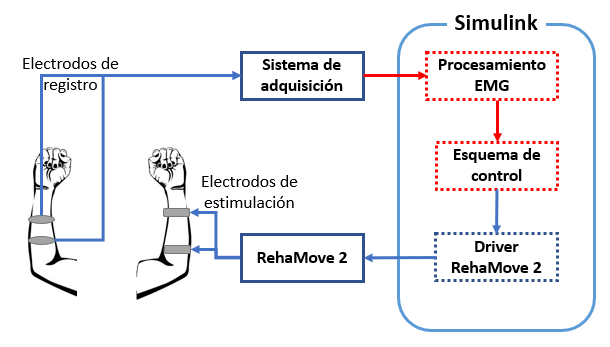
\includegraphics[scale=0.7]{SistemaPropuesto.png}
	\caption{Sistema propuesto para el proyecto. Líneas continuas representan entes de hardwares y líneas discontinuas representan entes de software. Elementos en rojo representan zonas de trabajo del proyecto.}
	\label{Figura: SistProp}
\end{figure}

\section{Adquisición de datos en Simulink}
Se utilizó el sistema Cyton Board (OpenBCI Inc., E.E. U.U. A.A.), el cual tiene una frecuencia de muestreo de 250 Hz, para realizar la adquisición de las señales de sEMG. Dicho sistema utiliza un chip ADS1299 (Texas Instruments) para realizar la conversión analógico-digital de las señales, el cual codifica los datos de cada muestra, utilizando complemento a 2, en un bus de datos esquematizado en la Figura \ref{Figura: BusOut}.

\begin{figure}[htbp]
\centering
	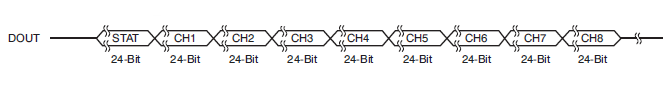
\includegraphics[scale=0.8]{Bus_Dat_Out_ADS.png}
	\caption{Estructura del bus de datos de salida del ADS1299}
	\label{Figura: BusOut}
\end{figure}

Para realizar la decodificación del bus de datos dentro de Simulink, se diseñó un subsistema encargado de la solicitud y decodificación de datos, para esto se utilizó el bloque \emph{Query Instrument} del \emph{Instrument Control Toolbox} para realizar la solicitud de datos, mientras que con bloques de la librería estándar de Simulink se realizó la decodificación de dichos datos.

El funcionamiento del subsistema responsable de la solicitud y decodificación de datos, esquematizado en la Figura \ref{Figura: DecoStream}, sigue los siguientes pasos:

\begin{enumerate}
	\item Realizar la adquisición de N muestras, lo cual generará un vector columna con dimensión (27*N,1).
	\item Aplicar un reshape a dicho vector para obtener una matriz con dimensión (27,N).
	\item Obtener la transpuesta de dicha matriz para obtener una matriz con dimension (N,27).
	\item Para cada canal, extraer de la matriz anterior las columnas asociadas a dicho canal de tal forma que se obtenga una submatriz con dimensión (N,3).
	\item Realizar una multiplicación matricial de dicha submatriz con un vector ponderador de tal forma que al final se obtenga un vector con dimensión (N,1) donde cada muestra n se encuentra en complemento a 2.
	\item Extraer del vector anterior las muestras en las que se encuentra codificado un número negativo (si el bit 23 de la muestra es 1 entonces se trata de un número negativo).
	\item Obtener el complemento a 1 de cada muestra del subvector obtenido, sumar 1 a cada muestra y por último multiplicar cada muestra por -1.
	\item Regresar los elementos del subvector al vector original.
\end{enumerate}

\begin{figure}[htbp]
\centering
	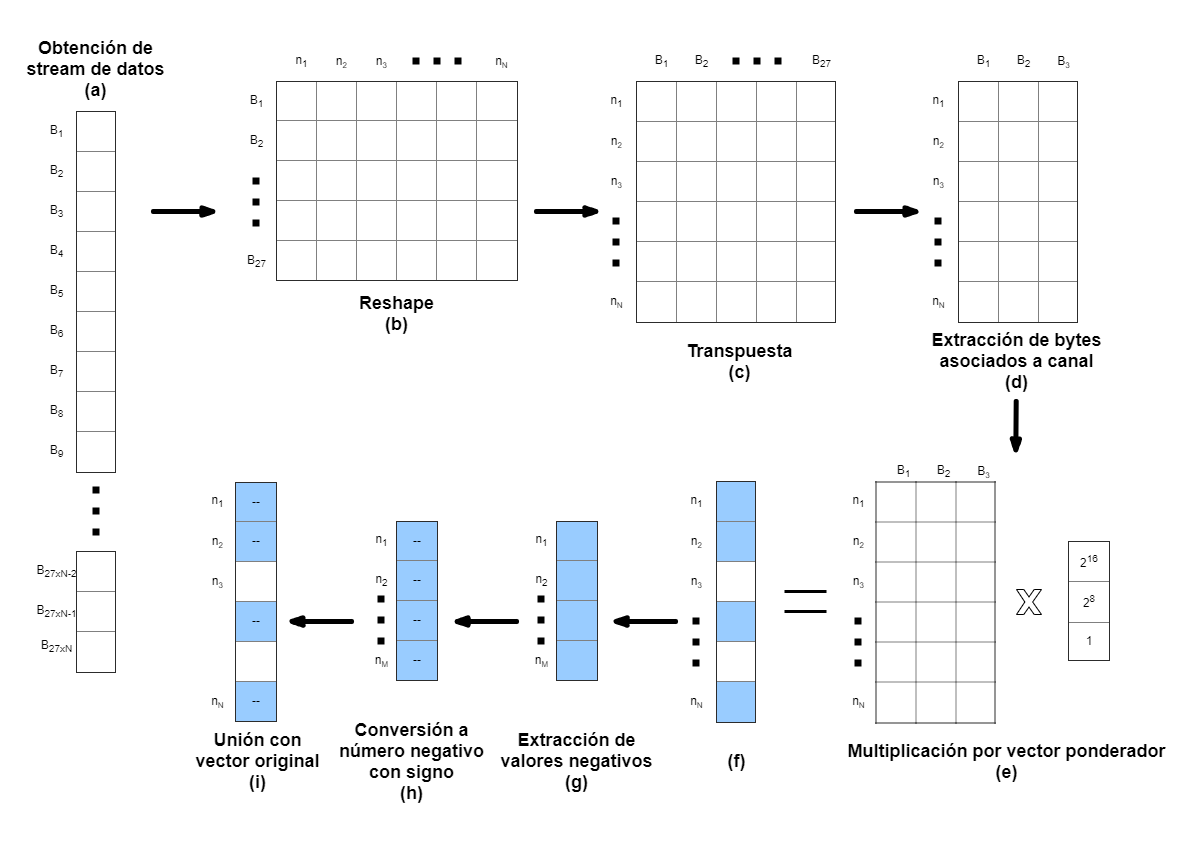
\includegraphics[scale=0.15]{DecoStream.png}
	\caption{Funcionamiento del subsistema decodificador del stream de datos}
	\label{Figura: DecoStream}
\end{figure}


La implementación final del subsistema diseñado en Simulink se observa en la Figura \ref{Figura: DecoSimuT}.

\begin{figure}[htbp]
	\centering
	\begin{subfigure}[htbp]{0.5\textwidth}
		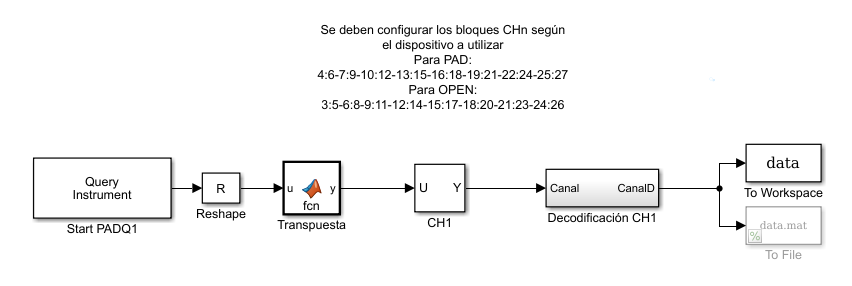
\includegraphics[width=\textwidth]{Read_Simu.png}
		\caption{Vista general del sistema diseñado para realizar adquisición y decodificación del stream de datos.}
		\label{Figura: readSimu}
	\end{subfigure}
	\begin{subfigure}[htbp]{0.5\textwidth}
		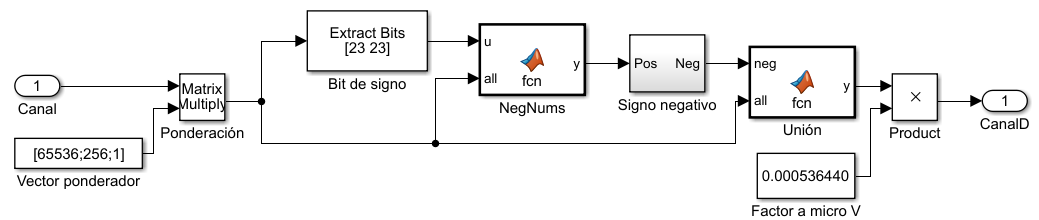
\includegraphics[width=\textwidth]{Deco_Simu.png}
		\caption{Vista interna del subsistema encargado de la decodificación del stream de datos.}
		\label{Figura: decoSimu}
	\end{subfigure}
	\caption{Sistema decodificador de stream de datos implementado en Simulink}
	\label{Figura: DecoSimuT}
\end{figure}

\section{Evaluación de bloque de adquisición y decodificación}
Para obtener una valoración sobre el funcionamiento del bloque diseñado dentro de Simulink para la adquisición y decodificación se generaron señales sintéticas dentro de MATLAB para que sirvieran como patrón de evaluación. Dichas señales consistieron en un banco de 5 senoidales a diferentes frecuencias (1 Hz, 5 Hz, 10 Hz, 20 Hz y 50 Hz (Figura \ref{Figura: SenPur})), dos senoidales de 50 Hz moduladas en amplitud con una exponencial decreciente (Figura \ref{Figura: ExpAte}) y una recta con pendiente negativa (Figura \ref{Figura: LinAte}), y una senoidal de 50 Hz modulada de tal forma que simule un contracción muscular que sube, se mantiene por un tiempo y baja (Figura \ref{Figura: Contra}). La duración de estas señales es de 5 segundos cada una, exeptuando la última que tiene una duración de 15 segundos, y todas se diseñaron con una frecuencia de muestreo de 250 Hz.

%Figura de senoidales MATLAB
\begin{figure}[htbp]
	\centering
	\begin{subfigure}[htbp]{0.4\textwidth}
		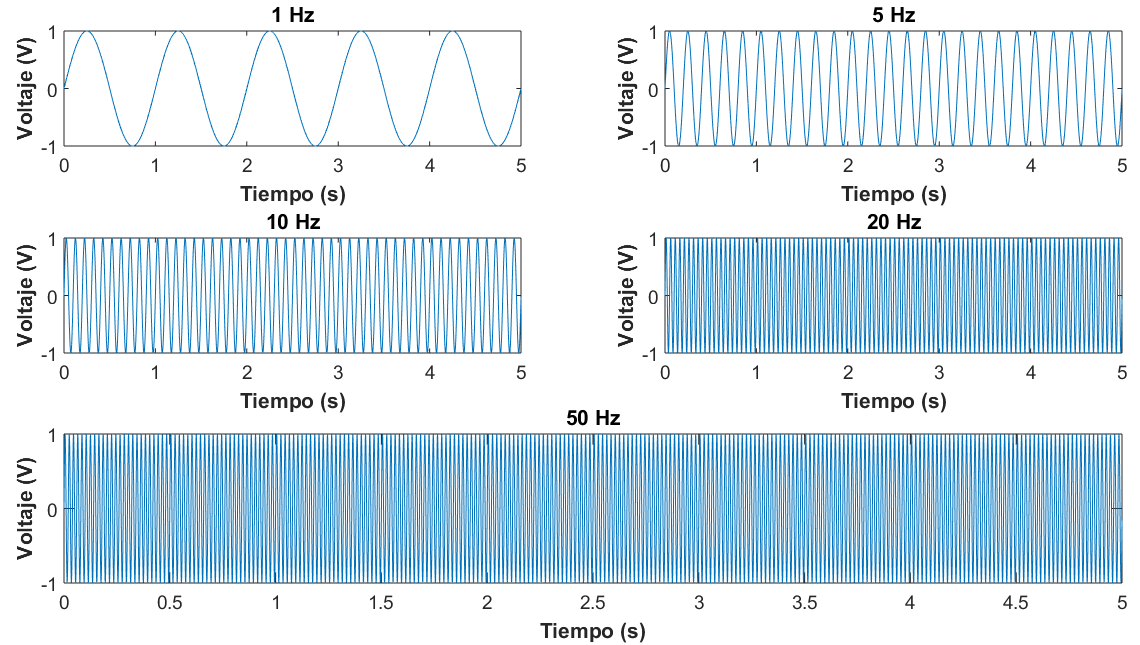
\includegraphics[width=\textwidth]{Sen_Pur.png}
		\caption{Senoidales puras a diferentes frecuencias}
		\label{Figura: SenPur}
	\end{subfigure}
	\hfill
	\begin{subfigure}[htbp]{0.4\textwidth}
		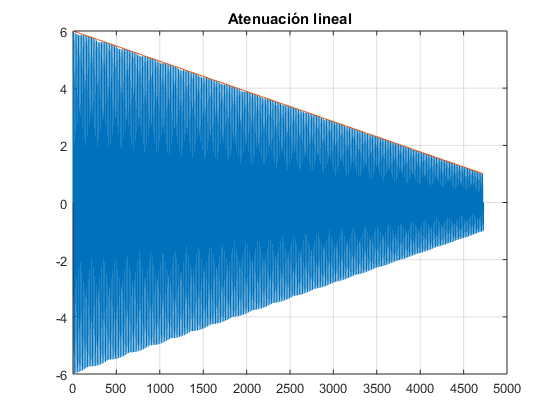
\includegraphics[width=\textwidth]{Lin_Ate.png}
		\caption{Senoidal de 50 Hz con atenuación lineal}
		\label{Figura: LinAte}
	\end{subfigure}
	\hfill
	\begin{subfigure}[htbp]{0.4\textwidth}
		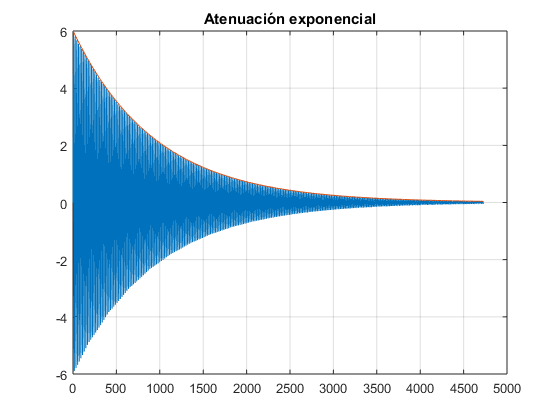
\includegraphics[width=\textwidth]{Exp_Ate.png}
		\caption{Senoidal de 50 Hz con atenuación exponencial}
		\label{Figura: ExpAte}
	\end{subfigure}
	\hfill
	\begin{subfigure}[htbp]{0.4\textwidth}
		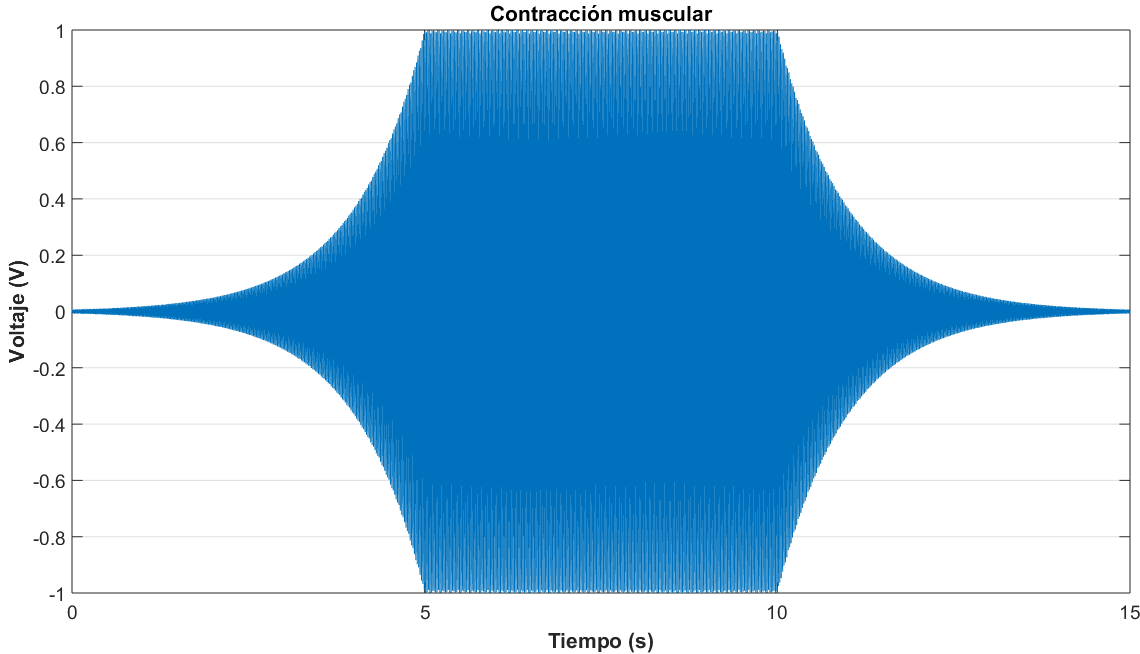
\includegraphics[width=\textwidth]{Contra.png}
		\caption{Senoidal de 50 Hz simulando una contracción muscular}
		\label{Figura: Contra}
	\end{subfigure}	
	\caption{Señales creadas para la evaluación del protocolo de comunicación}
	\label{Figura: SenalesEva}
\end{figure}

El proceso de evaluación se realizó de la siguiente manera:
\begin{enumerate}
	\item Utilizando un jack de audio de 3.5 mm, se conectó una punta a la salida de audio de la computadora, mientras que la otra punta se conectó al canal 1 del sistema de adquisición.
%	\item El canal 1 del prototipo de adquisición se configuró con una ganancia de 1 y se hablilitó el BIAS para dicho canal. La frecuencia de muestreo del prototipo se configuró a 1 kHz.
	\item Se inició la solicitud de datos utilizando el subsistema decodificador implementado en Simulink y se inició el contento de un cronómetro.
	\item Tras haber transcurridos 2 segundo en el cronómetro, se procedió a la reproducción de la señal tratándola como una señal de audio en MATLAB.
	\item Al marcar el cronómetro 10 segundos (20 segundos para la señal de larga duración), se detuvo la adquisición en el sistema de Simulink.
	\item Se calculó la métrica de correlación entre ambas señales como indicador de la calidad de la transferencia de datos.
\end{enumerate}

Se realizaron tres repeticiones de cada señal, obteniendo un total de 24 registros para la obtención de la correlación, dando un resultado de correlación promedio de 0.9615 $\pm$ 0.0604.

\section{Protocolo para registro de sEMG}
Para garantizar una repetibilidad en los registros de sEMG se implementó un protocolo para realizar la adquisición de dicha señal. Dicho protocolo tiene las caracteristicas mostradas a continuación:

\begin{itemize}
	\item Frecuencia de muestro de sistema de adquisición: 250 Hz.
	\item Canales 1 y 2 para realizar adquisición.
	\item Electrodos: Covidien H124SG
	\item Canal 1: Digitorum flexor
	\begin{itemize}
		\item Medir antebrazo de lado ventral de codo a muñeca.
		\item Palpar músculo al 25\% de la medida obtenida.
		\item Colocar dos electrodos separados 2 cm (Figura \ref{Figura: E_Cie}).
	\end{itemize}
	\item Canal 2: Digitorum extensor
	\begin{itemize}
		\item Medir antebrazo de lado dorsal de codo a muñeca.
		\item Palpar músculo al 50\% de la medida obtenida.
		\item Colocar dos electrodos separados 2 cm (Figura \ref{Figura: E_Ape}).
	\end{itemize}
	\item Referencia: Colocar electrodo en codo.
\end{itemize}

\begin{figure}[htbp]
	\centering
	\begin{subfigure}[htbp]{0.3\textwidth}
		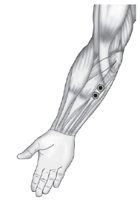
\includegraphics[width=\textwidth]{E_Cie.png}
		\caption{Ubicación de electrodos para digitorum flexor.}
		\label{Figura: E_Cie}
	\end{subfigure}
	\hfill
	\begin{subfigure}[htbp]{0.3\textwidth}
		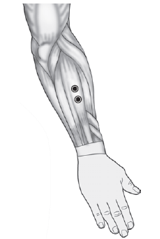
\includegraphics[width=\textwidth]{E_Ape.png}
		\caption{Ubicación de electrodos para digitorum extensor.}
		\label{Figura: E_Ape}
	\end{subfigure}
	\caption{Posicionamiento de electrodos para realizar registros de sEMG. Recuperado de \cite{Cavalcanti-Garcia2009}.}
	\label{Figura: E_sEMG}
\end{figure}

\section{Procesamiento de sEMG}

Se diseñaron tres filtros Butterworth para realizar el procesamiento de sEMG: un filtro pasa altas con frecuencia de corte de 15 Hz,para eliminar las variaciones en la línea base del registro; un filtro pasa bajas con frecuencia de corte de 100 Hz, para eliminar armónicos de 60 Hz y demás interferencias de alta frecuencia; y un filtro rechaza banda centrado en 60 Hz, para reducir la interferencia de la línea. Las gráficas de respuesta en frecuencia de estos filtros se muestran en las Figuras \ref{Figura: FiltroPA} a \ref{Figura: FiltroRB}.

\begin{figure}[htbp]
	\centering
	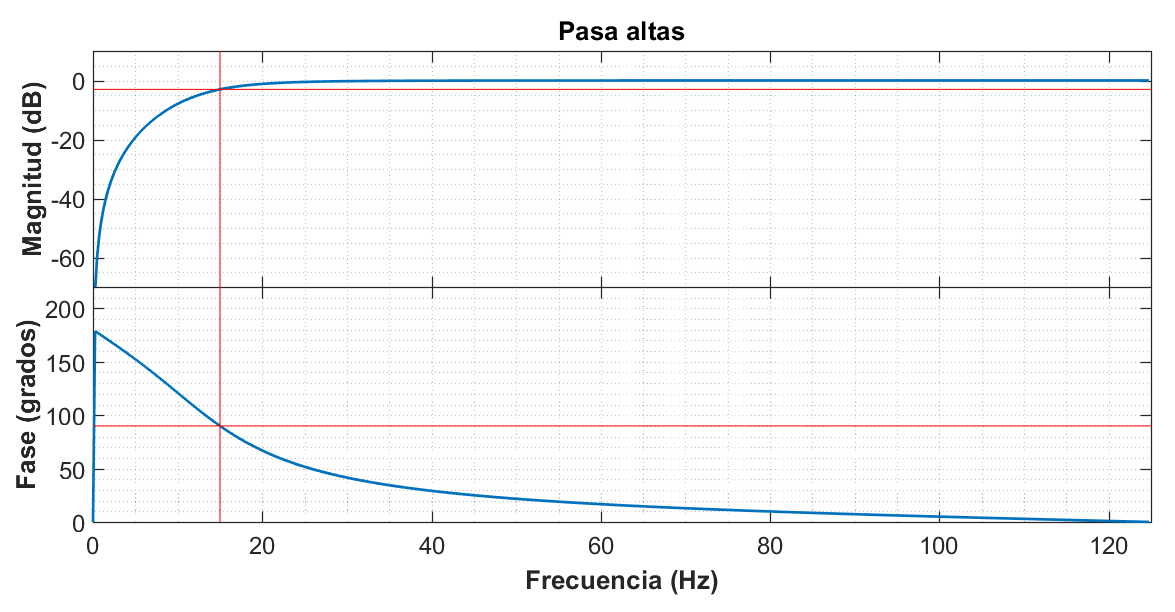
\includegraphics[width=0.7\textwidth]{FiltroPA15Hz_PADQ.png}
	\caption{Filtro pasa altas para conseguir línea base estable.}
	\label{Figura: FiltroPA}
	
	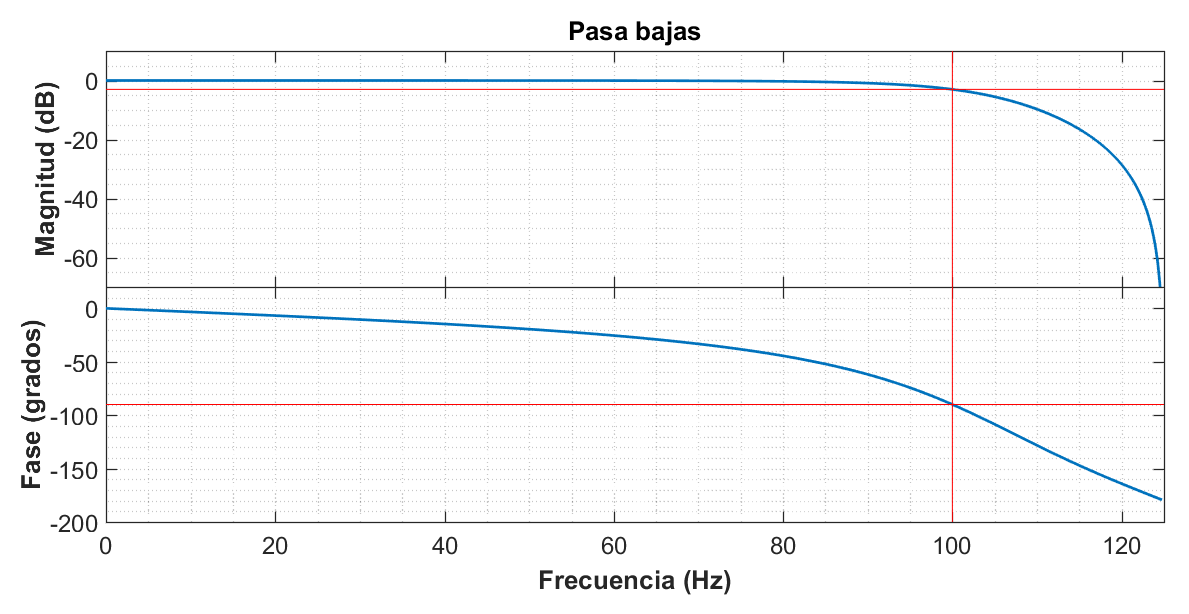
\includegraphics[width=0.7\textwidth]{FiltroPB100Hz_PADQ.png}
	\caption{Filtro pasa bajas para eliminar interferencias de alta frecuencia y armónicos de 60 Hz.} 
	\label{Figura: FiltroPB}
	
	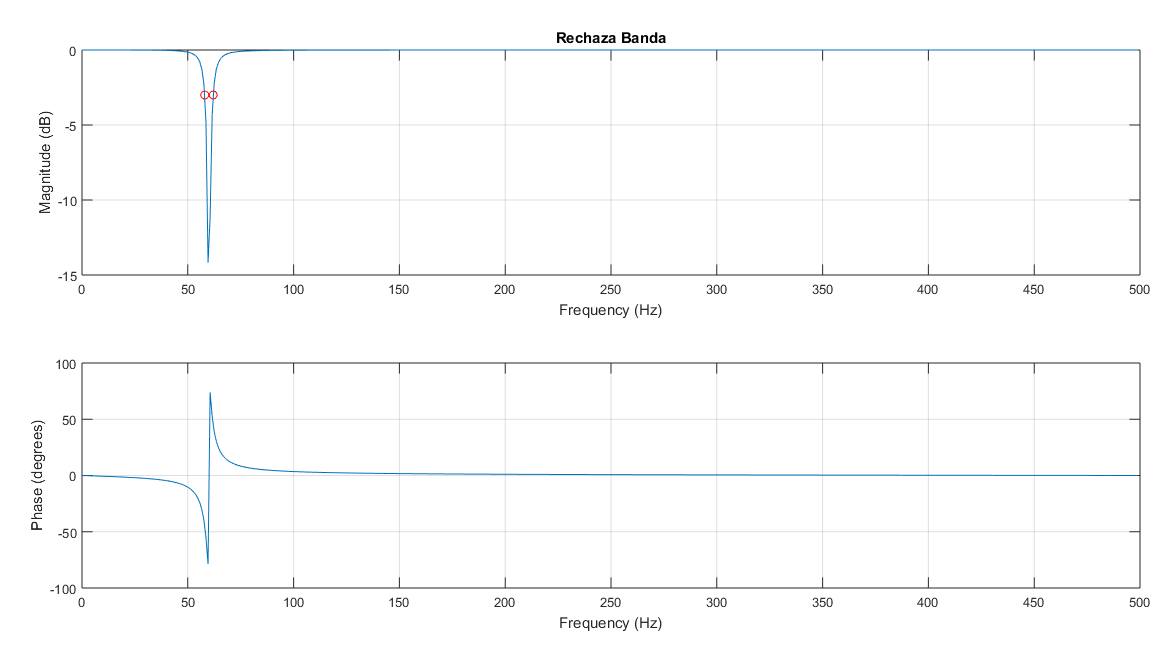
\includegraphics[width=0.7\textwidth]{FiltroRB_58_62_PADQ.png}
	\caption{Filtro rechaza banda para reducir interferencia de 60 Hz.}
	\label{Figura: FiltroRB}
\end{figure}

Se implementó dentro de Simulink un bloque responsable de obtener el valor RMS de ventanas de registro de 100 ms de sEMG para utilizar dicho descriptor de amplitud como señal de control. Adicionalmente se implementó un filtro de de mediana de 10 muestras (Ecuación \ref{Mediana}), el cual tiene como propósito conseguir una señal de RMS suavizada

\begin{equation}
	y[n] = mediana(x[n]:x[n-N])
	\label{Mediana}
\end{equation}

\newpage
\section{Esquema de control}
Se diseñó un sistema basado en una combinación de máquina de estados finitos con un control lineal. El sistema requiere de un proceso de calibración previa donde se obtienen 8 umbrales tras la repetición de 4 movimientos, dos umbrales corresponden a los valores RMS promedio de los dos canales de adquisición a lo largo de la tarea \emph{cierre de mano ligero}, otros dos corresponden a los valores RMS promedio de la tarea \emph{cierre de mano completo}, mientras que los 4 restantes corresponden a los valores RMS promedio de las tareas \emph{apertura de mano ligera} y \emph{apertura de mano completa}. {\color{red}AGREGAR FOTO DE POSTURAS DE MANOS}. Además, tras la calibración se obtiene también un factor denominado \emph{detector de movimiento}, el cual se obtiene tras calcular la diferencia promedio entre los canales de adquisición a lo largo de la tarea de apertura de mano. Adicionalmente se realiza una calibración de la estimulación eléctrica, la cual utiliza el sistema de colocación de electrodos de estimulación descrito en [{\color {red}ANA}], donde se obtiene los valores en amplitud de los umbrales motores y funcionales de las tareas de apertura y cierre de mano.

El detector de movimiento se utiliza para realizar el control por máquina de estados finitos (Figura \ref{Figura: FSM_control}), la cual consisten en determinar si la diferencia de amplitudes entre canales ha pasado el valor del detector de movimiento, si es así, el control prosigue con la tarea de apertura de mano, en caso contrario, el control procede a la tarea de cierre de mano.

\begin{figure}[htbp]
	\centering
	\includegraphics[scale=0.9]{FSM_control.png}
	\caption{Máquina de estados finitos encargada de la detección de movimiento e inicio del control lineal.}
	\label{Figura: FSM_control}
\end{figure}

Dentro del control de cada tarea, se utilizan los umbrales de las tareas ligeras para realizar la activación del control lineal, el cual modula la amplitud de la corriente eléctrica, del canal asociado al movimiento detectado, utilizando la recta descrita por la Ecuación \ref{Mapeo}, donde $A$ representa la amplitud que inyectará el estimulador eléctrico, $A_{max}$ es el umbral funcional de estimulación eléctica, $A_{min}$ es el umbral motor de estimulación eléctica, $D$ representa el valor RMS actual, mientras que $D_{max}$ y $D_{min}$ representan los umbrales RMS de la tarea completa y ligera del canal asociado al movimiento detectado (canal 1 para cierre de mano y canal 2 para apertura de mano). Adicionalmente se aplica la función máximo entero a la recta debido a que el dispositivo de estimulación eléctrica sólo admite valores enteros, y también se aplica un criterio de saturación de corriente eléctrica para evitar que tras una contracción muscular muy fuerte se genere un valor de amplitud de corriente eléctrica dañino para el sujeto.

\begin{equation}
	A = \frac{A_{max} - A_{min}}{D_{max} - D_{min}}(D - D_{min}) + A_{min}
	\label{Mapeo}
\end{equation}


\chapter{Resultados}
%%RESULTADOS

\section{Adquisición de datos}
Tras realizar la evaluación del subsistema de adquisición descrito en la sección \ref{Sec: Adquisicion} utilizando el procedimiento detallado en la sección \ref{Sec: EvalAdquisicion}, se obtuvo un valor de correlación promedio de 0.915 $\pm$ 0.0604, el cual se obtuvo de un total de 40 registros realizados (3 repeticiones de cada una de las señales que conforman el banco de señales para evaluación de la adquisición). En la Figura \ref{Figura: ValProCum} se puede observar una comparación entre la señal patrón y la señal adquirida con el subsistema diseñado en Simulink.


%Tras adquirir las señales patrón para la evaluación del bloque de adquisición descritas en la metodología, se calculó la métrica de correlación entre las señales adquiridas y las patrón, buscando traslapar una sobre otra como se muestra en la Figura \ref{Figura: ValProCum}. Al tener el valor de correlación para cada registro se obtuvo como resultado una correlación promedio de 0.9615 $\pm$ 0.0604, valor que sirve como indicador de la calidad del bloque diseñado para la adquisición y decodificación de datos.

%Senoidal obtenida tras para evaluación
\begin{figure}[htbp]
	\centering
	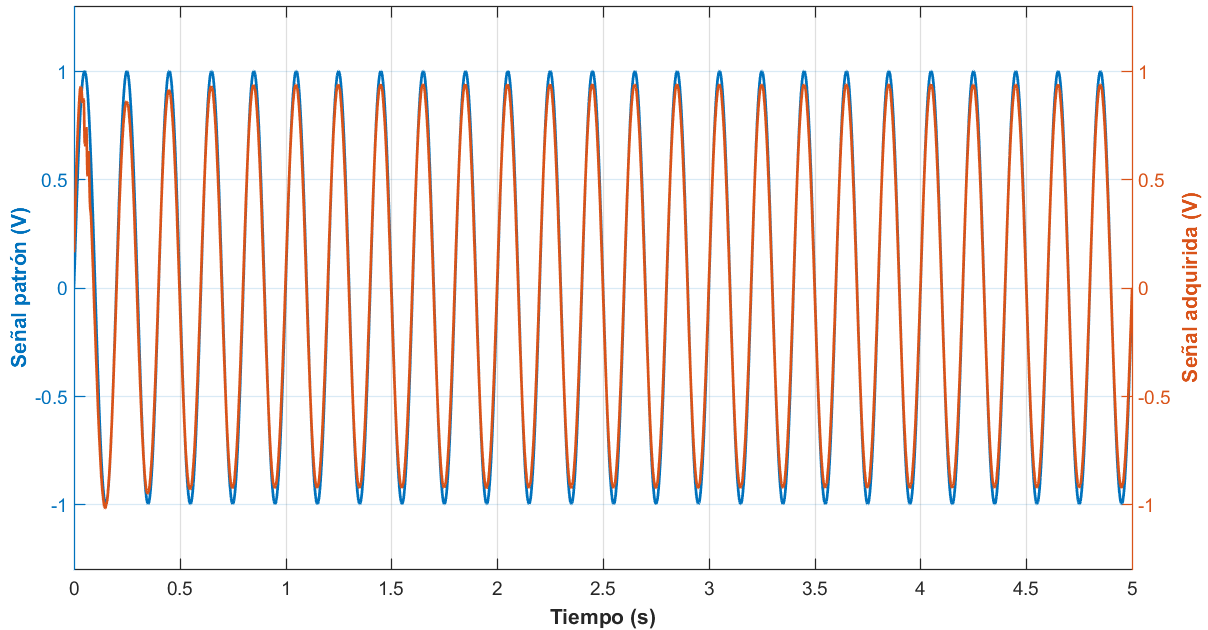
\includegraphics[width=\textwidth]{ValProCum.png}
	\caption[Comparación entre señales para evaluación de adquisición.]{Comparación entre señales para evaluación de adquisición. Señal patrón generada en MATLAB (azul). Señal adquirida mediante el subsistema de adquisición diseñado en Simulink (Rojo).}
	\label{Figura: ValProCum}
\end{figure}


\section{Procesamiento de sEMG}
El esquema de filtrado utilizado (filtro pasa altas, filtro pasa bajas y filtro rechaza banda), al igual que el procesamiento para obtención del RMS suavizado, se pusieron a prueba fuera de línea con 10 sujetos (6 hombres y 4 mujeres) sanos de edades entre 20 y 24 años.

La Figura \ref{Figura: Filtrado} muestra una comparación entre los canales de sEMG adquiridos para las pruebas de procesamiento y el resultado de su filtrado fuera de línea.

En la Figura \ref{Figura: RMS} se muestra un ejemplo del resultado del procesamiento para obtención de RMS suavizado.

%Utilizando los registros de calibración se probaron los filtros diseñados, obteniendo como resultado notorio la estabilización de la línea base de cada registro. En la Figura \ref{Figura: Filtrado} se muestra una comparación entre los registros crudos y filtrados de ambos canales adquiridos durante el entrenamiento.

\begin{figure}[htbp]
	\centering
	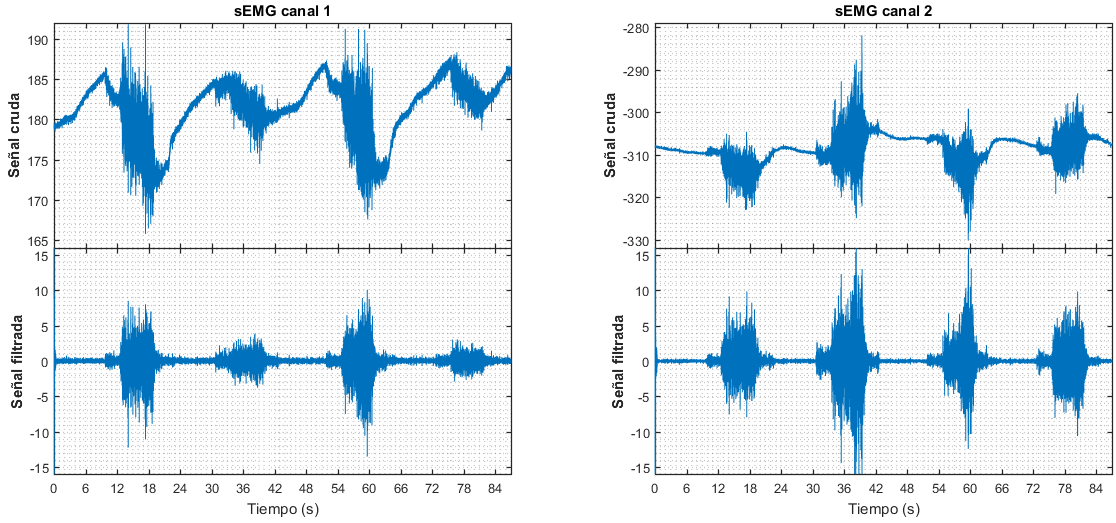
\includegraphics[width=0.8\textwidth]{Filtrado.png}
	\caption{Ejemplo representativo del funcionamiento del esquema de filtrado diseñado.}
	\label{Figura: Filtrado}
\end{figure}

%Con los registros ya filtrados se obtuvo el valor RMS a lo largo de todo el registro utilizando ventanas de 100 ms, dando como resultado una envolvente discreta de sEMG para cada canal. En la Figura \ref{Figura: RMS} se muestran los registros de sEMG filtrados con sus respectivas envolventes discretas de RMS y marcadores de la acción solicitada al sujeto durante el entrenamiento.

\begin{figure}[htbp]
	\centering
	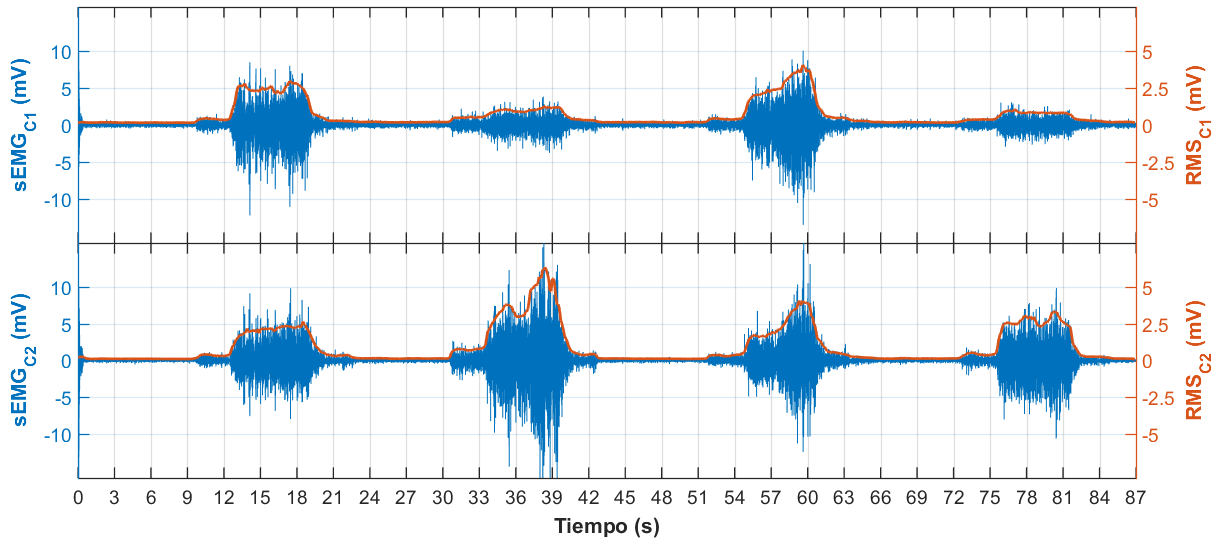
\includegraphics[width=\textwidth]{RMS.png}
	\caption[Ejemplo representativo de la obtención de envolvente de RMS]{Ejemplo representativo de la obtención de envolvente de RMS. En azul, los registros de sEMG. En rojo, las envolventes de RMS.}
	\label{Figura: RMS}
\end{figure}


\section{Sistema de control}
El sistema completo se puso a prueba con un sujeto varón sano de 22 años de edad, en el cual presentaron resultados satisfactorios. Relacionado a la validación fuera de línea, el algoritmo para la clasificación de los movimientos obtuvo un porcentaje de acierto del 81$\%$. La Figura \ref{Figura: MapOff} muestra el resultado de la prueba para la validación fuera de línea. Respecto a la prueba de validación en línea, en esta demostró una respuesta del sistema de acuerdo a lo esperado. La Figura \ref{Figura: MapOn} presenta un segmento de las señales obtenidas tras la realización de la prueba en línea. En relación a la tarea objetivo, el sistema logró llevar a cabo la modulación de la estimulación eléctrica de forma satisfactoria, con un notable retardo del sistema, el cual al medirlo como se describe en la sección \ref{Sec: TareaObj}, se obtuvo un valor de retardo de 2.3 $\pm$ 0.3553 s. La Figura \ref{Figura: Retardo} muestra un acercamiento a las señales obtenidas al termino de la tarea objetivo, donde es notorio el retardo entre la generación de la señal patrón y el inicio de la modulación de estimulación eléctrica.

Respecto a la tarea funcional, este se logró llevar a cabo sin complicaciones en el sujeto de prueba antes mencionado, el cual pudo realizar por completo la tarea. Las Figuras \ref{Figura: Fun_A_1} a \ref{Figura: Fun_A_2} muestran momentos en los que el sujeto llevó a cabo la tarea funcional.
%Previo a realizar pruebas del esquema de control en línea, este se probó fuera de línea, aprovechando los registros de calibración. Para estas pruebas se diseñó un script en MATLAB que obtiene los parámetros necesarios del esquema de control de la misma forma que los arroja la calibración. Una vez obtenidos dichos parámetros se configura con ellos al esquema de control y se realiza una prueba fuera de línea donde con cada ventana de sEMG se obtiene un valor de RMS el cuál es sometido al esquema de control y arroja un valor de amplitud para el canal asociado al movimiento detectado. Tras probar el esquema de control con tres registros distintos de calibración se obtuvo un porcentaje de acierto del 81$\%$ en la identificación correcta de los movimientos de cierre, apertura y descanso de mano.

%En la Figura \ref{Figura: MapOff} se muestra el resultado de  una prueba exitosa del esquema de control fuera de línea, donde se observa que el esquema de control diseñado suele presentar errores en la identificación de los segmentos iniciales y finales de la tarea apertura de mano.

\begin{figure}[htbp]
	\centering
	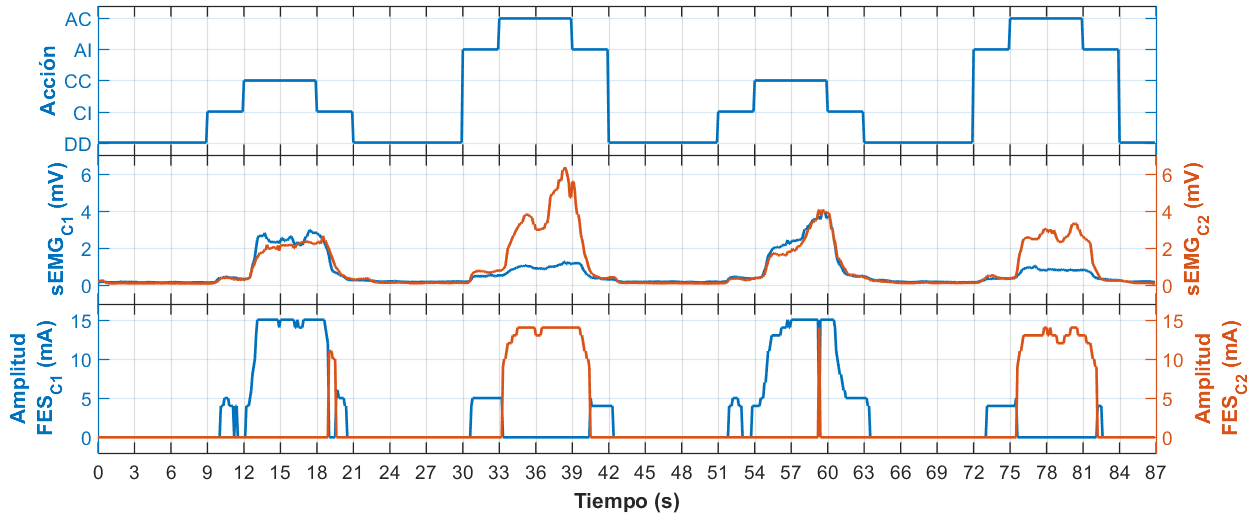
\includegraphics[width=\textwidth]{MapOff.png}
	\caption[Ejemplo representativo exitoso del funcionamiento fuera de línea del sistema de control]{Ejemplo representativo exitoso del funcionamiento fuera de línea del sistema de control. Arriba: Envolventes de sEMG (Azul: canal 1. Rojo: canal 2). Centro: Amplitudes de estimulación eléctrica (salida del sistema de control) (Azul: canal 1. Rojo: canal 2). Abajo: Marcadores de acción solicitada al sujeto (descanso (DD), pinza gruesa incompleta (CI), pinza gruesa completa (CC), apertura incompleta (AL), apertura completa (AC)).}
	\label{Figura: MapOff}
\end{figure}

%\newpage
%Para la prueba en línea se configuró el modelo de Simulink con los datos obtenidos tras la calibración, y se solicitó al sujeto realizar el seguimiento de un par de señales trapezoidales que le indicarían el tipo de movimiento que tendría que lograr. Cuando la trapezoidal estuviera en cero, tendría que mantenerse en descanso; en la pendiente positiva de la trapezoidal tendría que realizar una transición de descanso hacia el movimiento completo solicitado; en la meseta de la trapezoidal tendría que mantener el movimiento completo solicitado; y en la pendiente negativa de la trapezoidal tendría que realizar una transición del movimiento completo solicitado hacia descanso.

%En la Figura \ref{Figura: MapOn} se muestra un segmento de una de las pruebas exitosas realizadas en línea. En dicha figura se puede observar que existe un retardo entre la trapezoidal y la respuesta del sistema de control, el cual es la suma del retardo que genera el procesamiento de la señal, el retardo ocasionado por el esquema de control, y el tiempo de respuesta del sujeto a la indicación de la trapezoidal.

\begin{figure}[htbp]
	\centering
	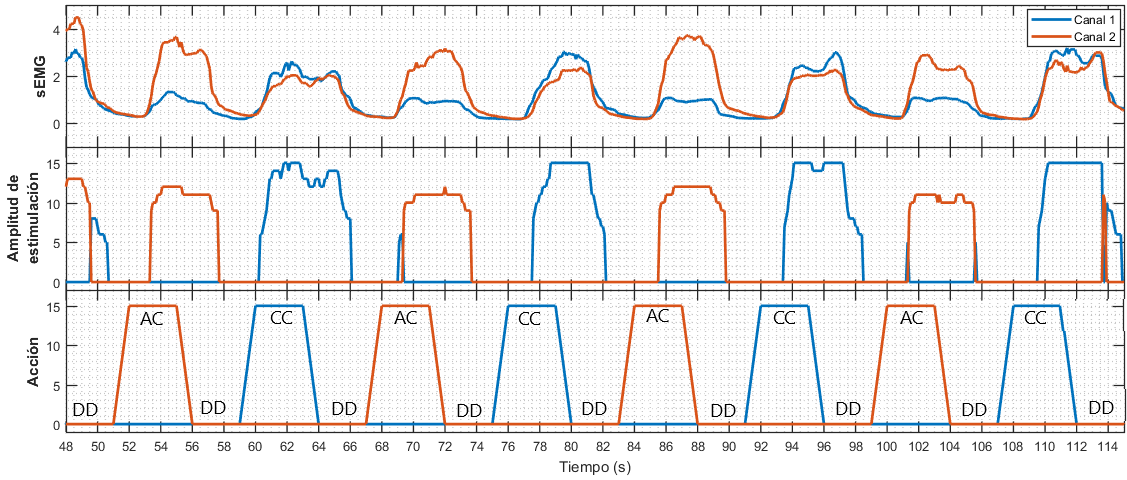
\includegraphics[width=\textwidth]{MapOn.png}
	\caption[Segmento de prueba representativa exitosa del funcionamiento en línea del sistema de control]{Segmento de prueba representativa exitosa del funcionamiento en línea del sistema de control.  Arriba: Envolventes de sEMG (Azul: canal 1. Rojo: canal 2). Centro: Amplitudes de estimulación eléctrica (salida del sistema de control) (Azul: canal 1. Rojo: canal 2). Abajo: Señal trapezoidal patrón indicadora de tarea a seguir (descanso (DD), pinza gruesa (CC), apertura completa (AC)).}
	\label{Figura: MapOn}
\end{figure}

%Para obtener el valor del retardo total se midió el tiempo existente entre el inicio de la pendiente positiva de la señal indicadora (trapezoidal) y la activación de la estimulación eléctrica. Al promediar los tiempos obtenidos a lo largo de las pruebas realizadas en línea se obtuvo un valor de 2.3 $\pm$ 0.3553 s.

%En la Figura \ref{Figura: Retardo} se muestra un acercamiento a las señales obtenidas en una prueba representativa de las pruebas realizadas en línea. Se muestran una sobre otra para visualizar el retardo existente entre el inicio de la señal indicadora y la activación de la estimulación eléctrica.

\begin{figure}[htbp]
	\centering
	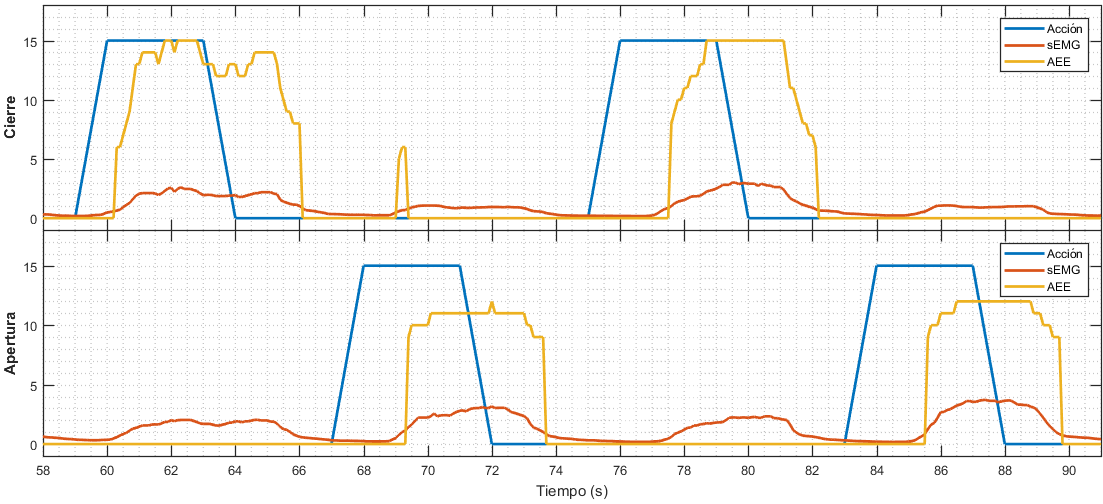
\includegraphics[width=\textwidth]{Retardo.png}
	\caption[Segmento de prueba representativa de tarea objetivo]{Segmento de prueba representativa de tarea objetivo. Se muestran las diferentes señales asociadas a cada movimiento una sobre otra para visualizar el retardo existente. Arriba: Señales para movimiento pinza gruesa completa. Abajo: Señales para movimiento apertura completa. En azul se muestra la señal trapezoidal patrón del movimiento a seguir. En rojo se muestra la envolvente de sEMG. En amarillo se muestra la amplitud de estimulación eléctrica (salida del sistema control).}
	\label{Figura: Retardo}
\end{figure}

%Posturas manos
\begin{figure}[htbp]
	\centering
	\begin{subfigure}[htbp]{0.45\textwidth}
		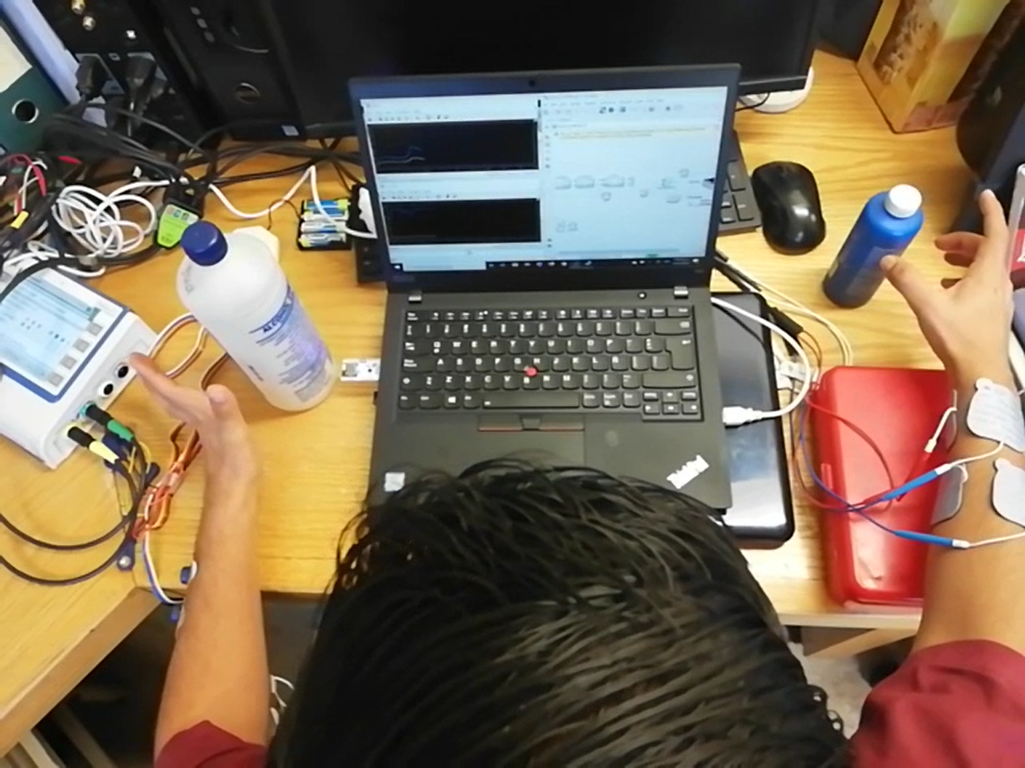
\includegraphics[width=\textwidth]{Funcional_Apertura_1.png}
		\caption{Apertura de mano para tomar objeto.}
		\label{Figura: Fun_A_1}
	\end{subfigure}
%	\hfill
	\begin{subfigure}[htbp]{0.45\textwidth}
		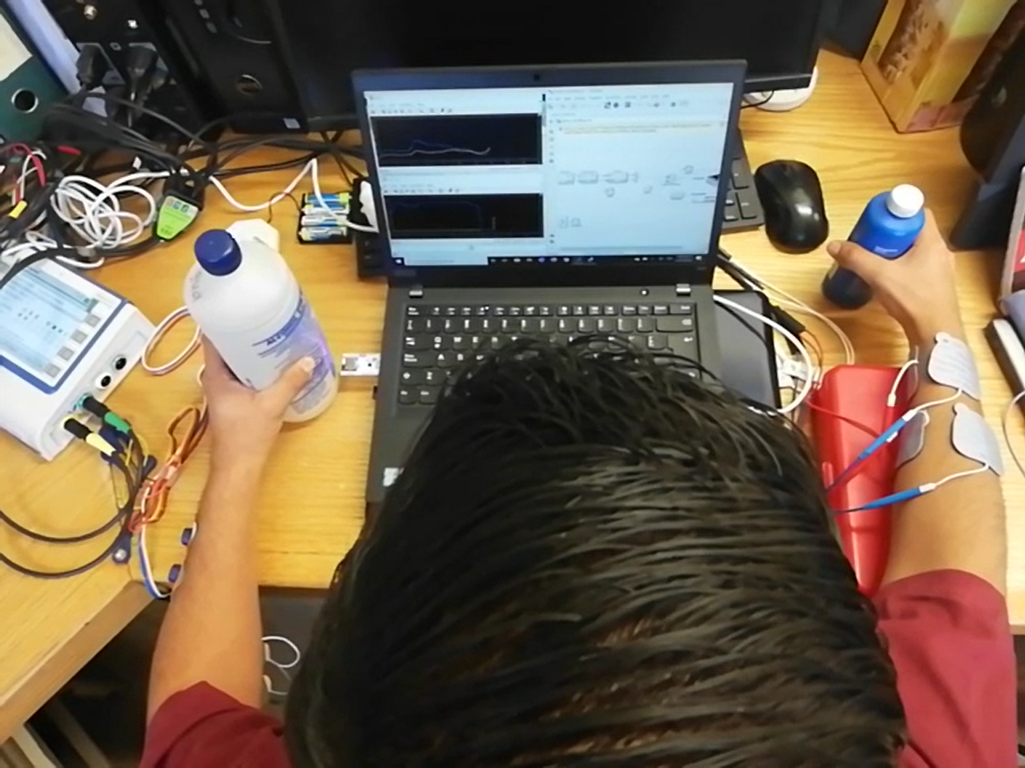
\includegraphics[width=\textwidth]{Funcional_Cierre.png}
		\caption{Pinza gruesa con objeto tomado.}
		\label{Figura: Fun_C}
	\end{subfigure}
%	\hfill
	\newline
	\begin{subfigure}[htbp]{0.45\textwidth}
		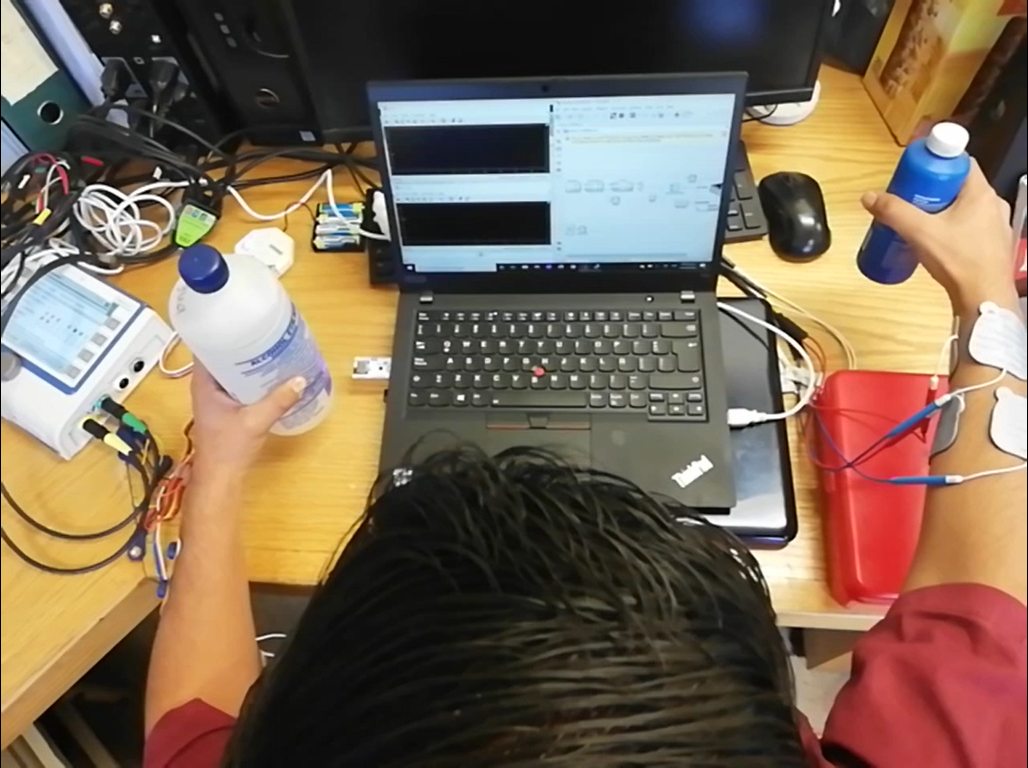
\includegraphics[width=\textwidth]{Funcional_Levantar.png}
		\caption{Levantamiento de objeto para trasladarlo.}
		\label{Figura: Fun_L}
	\end{subfigure}
%	\hfill
	\begin{subfigure}[htbp]{0.45\textwidth}
		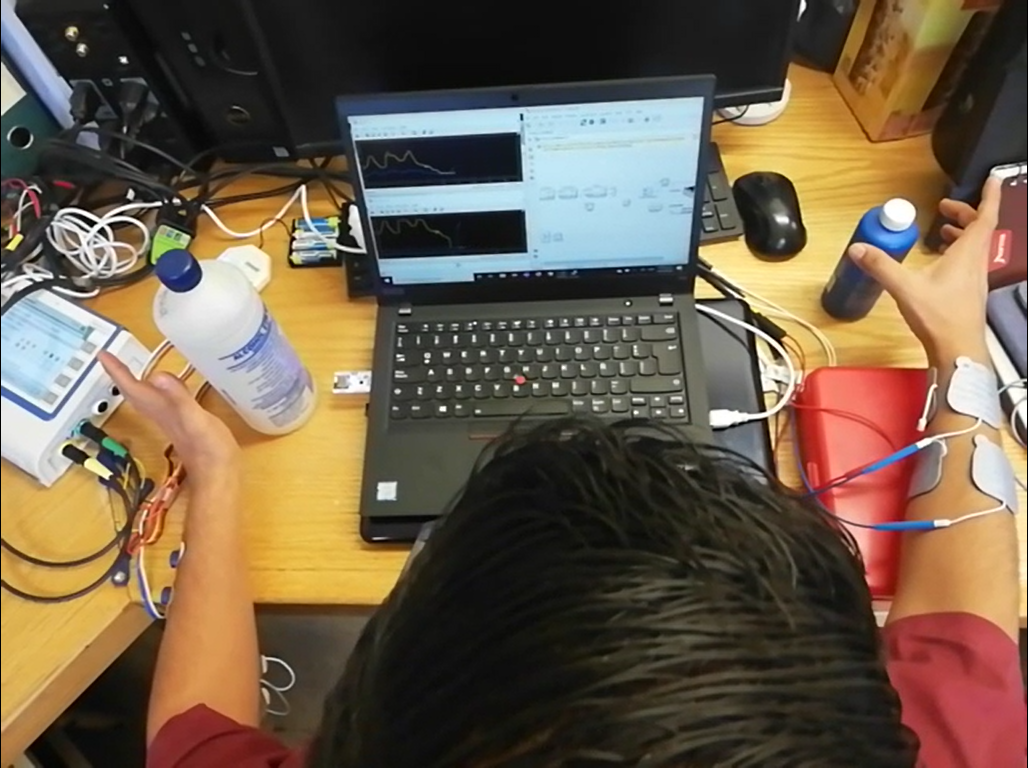
\includegraphics[width=\textwidth]{Funcional_Apertura_2.png}
		\caption{Apertura de mano para soltar objeto posterior a su traslado.}
		\label{Figura: Fun_A_2}
	\end{subfigure}
	\caption{Momentos de sujeto realizando tarea funcional.}
	\label{Figura: TareaFuncional}
\end{figure}

\chapter{Discusión y conclusiones}
Considero que el trabajo que he realizado hasta el momento es apenas casi la mitad del todo.

Falta terminar la evaluación del protocolo de comunicación, y la verdad siento que, como me lo mencionó Jorge, puede que la idea de generar la señales utilizando la tarjeta de audio de la computadora no sea la mejor para señales de baja frecuencia, así que quizás se podría tomar solamente una señal que se encuentre dentro del ancho de banda del prototipo y que la tarjeta de audio sea capaz de generarla, la cuál podría ser quizás una senoidal de 30 o 40 Hz, esto porque el espectro audible empieza en 20 Hz y la tarjeta de audio debería ser capaz de generar dicha señal.

En cuanto al procesamiento del sEMG creo que se debería de definir ya el tipo de filtro a utilizar, y creo que podríamos optar por una de las opciones que he encontrado en otros trabajos que utilizan el sEMG como control.

En cuanto al descriptor de amplitud creo que el RMS podría ser el adecuado, y creo que para lograr que dicho valor sea más estable la solución podría ser incrementar la ventana de registro y también pienso que el mapeo podría solucionar el problema de la estabilidad.

El mapeo inicialmente lo llegué a probar con una ecuación de una recta, pero de eso me di cuenta que puede que este tipo de mapeo genere ciertos problemas, ya que por ejemplo, con un RMS de 15.5 me generaría una corriente de 1 mA, pero con 15.6 de RMS generaría una corriente de 2 mA y ese cambio podría ser brusco para el paciente (como lo hemos visto lo cambios no tienen el mismo efecto en todos los pacientes).

Del sensor de fuerza tengo mis dudas sobre si tendré tiempo para lograr implementarlo, ya que siento que encontrar el mapeo adecuado para el proyecto me podría llevar más tiempo del que creía. Quizás y sería buena idea optar por un lazo cerrado donde sea el mismo sujeto el que controle el momento en el cuál la estimulación eléctrica es suficiente para realizar la tarea.

Otra cosa muy importante es que hace falta por definir la tarea a realizar, y creo que antes de continuar con todo lo demás deberíamos definir bien como va a ser la tarea a realizar.

\renewcommand{\bibname}{Referencias}
\bibliographystyle{acm}
\bibliography{11_biblio}

\end{document}